%% Seminar deck: Parsimonious yield curve modeling in less-liquid markets
%% (FAME|GRAPE Working Paper #53). House style, academic register.
\documentclass[aspectratio=169,11pt]{beamer}
\usepackage{beamerthemeyc}
\renewcommand{\deckfootertitle}{Dec · Parsimonious yield curve modeling in less-liquid markets · GRAPE WP \#53}

\begin{document}

% 1 ---------------------------------------------------------------------------
\begin{frame}[plain]
  \vspace{2mm}
  {\ttfamily\scriptsize\color{ycmuted}SEMINAR DECK · YIELDCARTOGRAPHY.COM}\\[-0.3em]
  {\color{ycrule}\rule{\textwidth}{0.5pt}}
  \vspace{4mm}

  {\fontsize{19}{23}\selectfont\bfseries\color{ycink}Parsimonious yield curve modeling\\in less-liquid markets.\par}
  \vspace{2mm}
  {\normalsize\color{ycmuted}The liquidity-weighted Nelson-Siegel-Svensson framework (LW-NSS).\par}
  \vspace{6mm}
  {\small\bfseries Marcin Dec\par}
  {\footnotesize\color{ycmuted}Kozminski University \& FAME|GRAPE, Warsaw\par}
  \vspace{3mm}
  {\ttfamily\scriptsize\color{ycaccent}FAME|GRAPE Working Paper \#53 · grape.org.pl/publications/wps\par}
  \vfill
  \raisebox{-1mm}{
\includegraphics[height=6mm]{kozminski_logo.png}}\hspace{5mm}
  \raisebox{-1mm}{
\includegraphics[height=6mm]{grape_logo.png}}\hspace{5mm}
  \raisebox{-1mm}{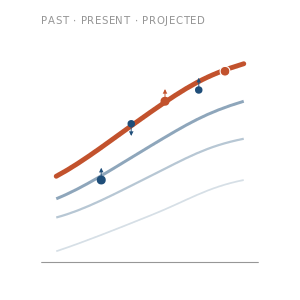
\includegraphics[height=6mm]{yc_logo.png}}
  \hfill{\ttfamily\scriptsize\color{ycmuted}NCN Preludium UMO-2020/37/N/HS4/02202}
\end{frame}

% 2 ---------------------------------------------------------------------------
\begin{frame}{Motivation}
  \kicker{Heteroskedastic observation noise across bonds}
  \begin{itemize}
    \item On a less-liquid sovereign curve, bond-level observation noise is
          strongly heterogeneous: daily turnover varies across issues by
          orders of magnitude, and a fixing on a rarely traded bond is a far
          noisier signal of the fundamental yield than one on a benchmark
          issue.
    \item Practitioners have long weighted parametric curve fits by turnover
          on intuition; the weighting scheme itself has lacked a
          microstructure foundation.
    \item Contribution: an explicit derivation of the efficient weight matrix
          for the Nelson--Siegel--Svensson fit from a dealer-market model of
          the fixing, and its empirical validation on the 21-year Polish
          panel.
  \end{itemize}
\end{frame}

% 3 ---------------------------------------------------------------------------
\begin{frame}{The estimator}
  \kicker{Weighted NSS in yield space}
  \small The zero curve follows Svensson (1994):
  \[ y(\tau;\theta) = \beta_0
     + \beta_1 \tfrac{1-e^{-\tau/\tau_1}}{\tau/\tau_1}
     + \beta_2 \Big( \tfrac{1-e^{-\tau/\tau_1}}{\tau/\tau_1} - e^{-\tau/\tau_1} \Big)
     + \beta_3 \Big( \tfrac{1-e^{-\tau/\tau_2}}{\tau/\tau_2} - e^{-\tau/\tau_2} \Big) \]
  fitted by weighted least squares on the observed bond-level yields:
  \[ \hat\theta_t \;=\; \arg\min_\theta \sum_{i}
     w_i \left( y^{obs}_{it} - y(\tau_{it};\theta) \right)^2 \]
  \begin{itemize}
    \item The open question is the choice of $w_i$: equal weights, duration
          weights and ad-hoc turnover weights coexist in practice.
  \end{itemize}
\end{frame}

% 4 ---------------------------------------------------------------------------
\begin{frame}{Microfoundation: a yield-space dealer market}
  \kicker{Glosten-Milgrom (1985) adapted to the fixing}
  \begin{itemize}
    \item The fixing on bond $i$ is modelled as a dealer's posterior over the
          fundamental yield after a Glosten--Milgrom quoting process run in
          yield space; in the active-trading regime the posterior variance is
          proportional to $\kappa/\mu_i$, with $\mu_i$ the bond's turnover
          intensity.
    \item The efficient GLS weight is the inverse noise variance, hence
          \( w_i = \mu_i \): turnover weighting is the information-matrix
          optimum, up to the common constant $\kappa$.
    \item Modified duration does not enter the noise process of a yield
          quote; it appears only as the Jacobian of the price-to-yield
          transformation in price-space implementations.
  \end{itemize}
\end{frame}

% 5 ---------------------------------------------------------------------------
\begin{frame}{Monte Carlo evidence}
  \kicker{Efficiency under the calibrated noise process}
  \begin{itemize}
    \item Simulation experiments generate bond panels under the
          turnover-dependent noise process calibrated to the Polish market
          and compare equal-weight, duration-weight and turnover-weight NSS
          fits.
    \item The turnover-weighted estimator attains the lowest parameter and
          curve RMSE across the designs, including configurations with
          near-degenerate curvature ($\beta_3$ close to redundant), where
          parameter identification is weakest.
  \end{itemize}
\end{frame}

% 6 ---------------------------------------------------------------------------
\begin{frame}{Empirical validation: the 21-year Polish panel}
  \kicker{Refit of the full history}
  \begin{itemize}
    \item Refitting the daily Polish sovereign panel (BondSpot fixings,
          monthly Ministry of Finance turnover as the empirical $\mu_i$)
          reduces the 21-year mean absolute fit error by 1.6 bp relative to
          the equal-weight NSS, while preserving the fitted curvature.
    \item The improvement concentrates where the theory predicts: on dates
          and segments where the turnover distribution across bonds is most
          uneven, i.e.\ where heteroskedasticity is strongest.
  \end{itemize}
\end{frame}

% 7 ---------------------------------------------------------------------------
\begin{frame}{Downstream consequences}
  \kicker{Weights propagate}
  \begin{itemize}
    \item The fitted curve is an input to everything downstream: forwards,
          carry and roll-down computations, and affine term-structure
          estimation.
    \item The choice of weighting scheme therefore propagates into ACM
          term-premium estimates; the paper quantifies the wedge between
          weighting schemes at the standard tenors.
    \item For markets in the LLM cohort the message is methodological:
          curve-fitting weights are an identification choice with
          economically visible consequences, and they admit a derivation
          in place of a convention.
  \end{itemize}
\end{frame}

% 8 ---------------------------------------------------------------------------
\begin{frame}{Companion data and replication}
  \kicker{yieldcartography.com}
  \begin{itemize}
    \item Every curve on the site is an LW-NSS fit: daily since 2005, weights
          from BondSpot turnover and outstanding amounts, on
          \textcolor{ycaccent}{\ttfamily yieldcartography.com/curves}.
    \item Fit diagnostics (bond count, MAE) are published per date on the
          curves tab and on the cockpit's vintage row.
    \item The ACM--BRW term premia built on these curves update daily on
          \textcolor{ycaccent}{\ttfamily /term-premia/}.
  \end{itemize}
\end{frame}

% 9 ---------------------------------------------------------------------------
\begin{frame}[plain]
  \vspace{12mm}
  {\fontsize{27}{31}\selectfont\bfseries\color{ycink}Thank you.\par}
  \vspace{6mm}
  {\normalsize\color{ycink}Marcin Dec\par}
  {\small\color{ycmuted}Kozminski University \& FAME|GRAPE, Warsaw\\
   mdec@kozminski.edu.pl · ORCID 0000-0002-6220-8267\par}
  \vspace{5mm}
  {\ttfamily\footnotesize\color{ycaccent}%
   Dec, M. Parsimonious Yield Curve Modeling in Less-Liquid Markets.\\
   FAME|GRAPE Working Paper \#53 · grape.org.pl/publications/wps\par}
  \vspace{5mm}
  {\ttfamily\scriptsize\color{ycmuted}Research supported by the National
   Science Centre, Poland · Preludium UMO-2020/37/N/HS4/02202\par}
  \vfill
  \raisebox{-1mm}{
\includegraphics[height=6mm]{kozminski_logo.png}}\hspace{5mm}
  \raisebox{-1mm}{
\includegraphics[height=6mm]{grape_logo.png}}\hspace{5mm}
  \raisebox{-1mm}{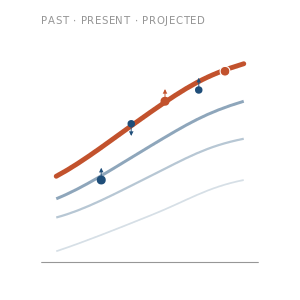
\includegraphics[height=6mm]{yc_logo.png}}
  \hfill{\ttfamily\scriptsize\color{ycmuted}yieldcartography.com/slides/lwnss/}
\end{frame}

\end{document}
